Write down some basics

\section{The Advanced LIGO Interferometers}

The Advanced LIGO (aLIGO) Interferometers are a pair of dual-recycled Michelson interferometers 
that employ Fabry-Perot cavities in their arms to increase the interaction time with a 
gravitational wave signal. 
Figure \ref{fig:aligo} shows a simplified layout of an aLIGO interferometer. 


\begin{figure}[ht!]
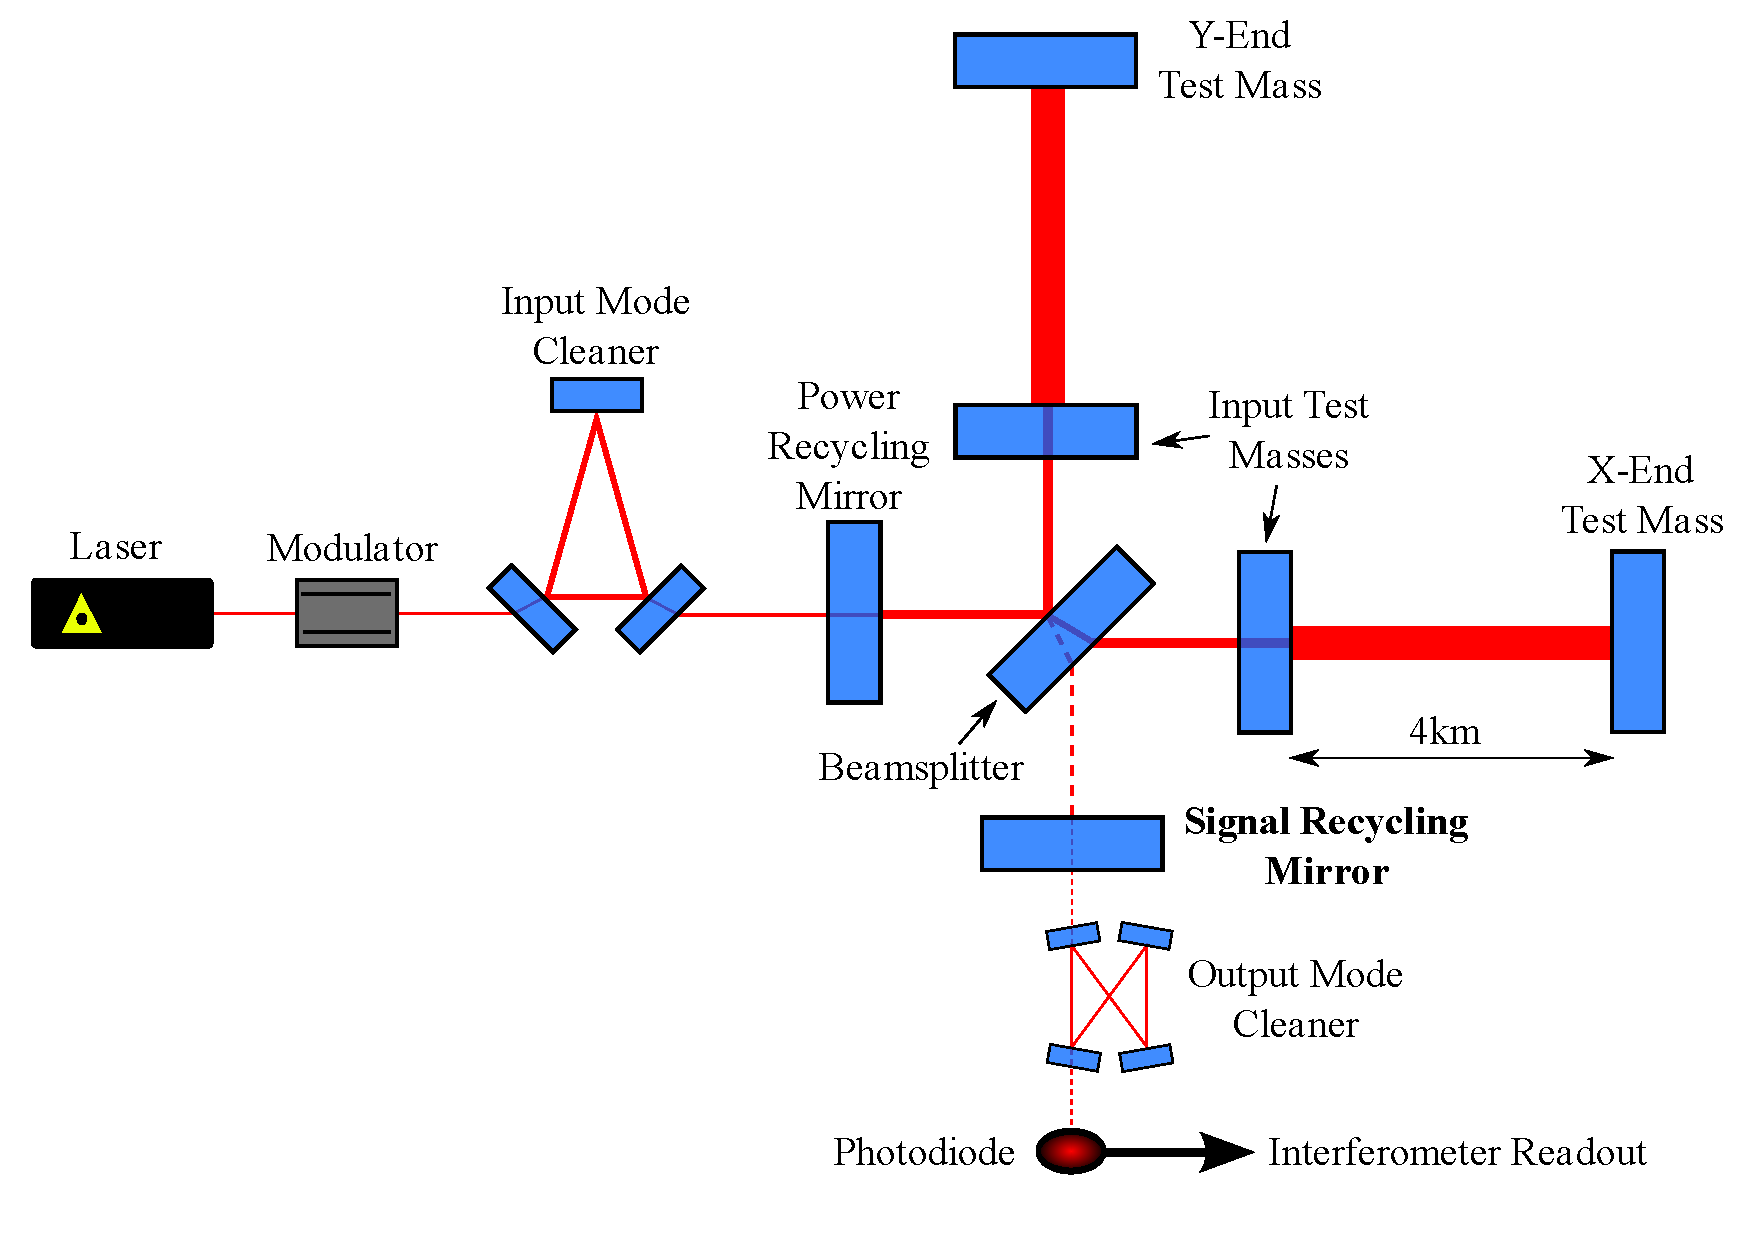
\includegraphics[width=\textwidth]{figures/introduction/ALIGO_layout}
\caption[Layout of Advanced LIGO]{Layout of Advanced LIGO}
\end{figure}\label{fig:aligo}

At the input to an aLIGO interferometer is a solid-state Nd:YAG laser that provides laser light 
at a wavelength of 1064 nm. Not included in Figure \ref{fig:aligo} are frequency and 
intensity stabilization control loops designed to provide as stable a laser source as 
possible for the experiment. This stabilized laser is called the pre-stabilized laser 
(PSL). The laser light is passed through a series of 
electro-optic modulators (EOM) where radio-frequency (RF) sidebands are generated 
and imparted onto the light. These RF sidebands are used to control auxiliary optical 
degrees of freedom in the interferometer. The beam is then passed through the 
input mode cleaner (IMC), which rejects higher order spatial modes of the beam 
and transmits a circular TEM00 mode to be used in the instrument.

Once the beam has been stabilized in frequency and intensity and the higher order 
optical modes have been stripped away, it is transmitted through the power 
recycling mirror and enters the vertex of the interferometer. In the vertex, 
the beam is split 50/50 by the beamsplitter. Half of the light is transmitted 
through the input test mass (ITM) of the X-arm and half of the light is transmitted 
through the ITM of the Y-arm. As mentioned previously, the aLIGO arms are not 
single bounce cavities; they are comprised of Fabry-Perot cavities that allow the 
light to circulate in the arm cavities multiple times. A small fraction of the 
light will be transmitted through the highly reflective end test mass (ETM) 
of the arm, but most of the light will transmit through the ITM and pass 
back into the vertex of the interferometer. 

When a gravitational wave passes through an aLIGO inteferometer, the distance
between the ITM and ETM of each arm is modulated, causing the light to have a
longer or shorter travel time as it traverses the arm. Since gravitational
waves expand space in one direction while the orthogonal direction contracts,     
the X- and Y-arms will experience differential changes in length. When light
from the arms is recombined at the beamsplitter, there will be a difference
in phase between the two beams as they have traveled different paths. The 
resulting light from this recombination of phase shifted beams is called the 
antisymmetric part of the output. The part of the beam that is recombined 
in phase is called the symmetric part of the output.

The beams returning from each arm are recombined at the beamsplitter. The 
symmetric part of the beam 
will be sent back toward the power recycling mirror. The power recycling mirror 
forms a resonant cavity with the ITMs, allowing for light at the symmetric 
port of the beamsplitter to be added coherently to incoming light from the PSL and 
increasing the effective power in the vertex. This increase in effective power 
is known as the power recycling gain. 

The antisymmetric part of the beam is sent toward the signal recycling mirror. 
The signal recycling cavity is used to tune the frequency response of the 
interferometer by adjusting the effective finesse of the coupled cavity 
formed by the signal recycling cavity and the arm cavities. 
If the light returning from the arms has accumulated some differential amount of 
phase as it traveled 
along the arms, perhaps from a gravitational wave modulating the length of each 
arm differentially, it will be transmitted through the signal recycling cavity 
and into the output mode cleaner (OMC). The OMC behaves similarly to the IMC, 
stripping away higher order optical modes and isolating the TEM00 mode of the 
beam. The transmitted, mode cleaned signal is then read out using a homodyne 
detection scheme on a DC photodiode. 

\subsection{DC Readout}

When a gravitational wave modulates the length of an arm cavity, the light 
traveling in that arm experiences a phase modulation. This phase modulation 
can be visualized by picturing the beam in frequency space. In figure 
\ref{fig:omc-freq}, the carrier beam frequency is designated as $f_0$. 
The phase modulation due to 
a gravitational wave signal introduces a frequency sideband at the 
gravitational wave frequency, which is in the 30-2000 Hz range. 
The 
RF sidebands used for auxiliary optical cavity control are offset from the 
carrier frequency by 9, 24, and 45 MHz. 
The RF sidebands, which in a 
homodyne detection scheme would only contribute shot noise to the output signal, 
are rejected by the OMC. The gravitational wave sidebands, however, are at a 
low enough frequency offset that they are within the cavity pole of the OMC 
and are allowed to transmit through the cavity.

Since the OMC DC photodiode measures power, it measures the square of the 
incident optical field and witnesses beat frequencies between different 
components of the light. If the RF sidebands have been filtered out by 
the OMC, the only remaining beat note will be that of the carrier beam ($f_0$) 
beating against the gravitational wave sideband ($f_0 + f_{GW}$). This beat note will 
appear as the difference in frequency between the two optical fields, 
leaving behind a signal in the 30-2000 Hz range ($f_{GW}$) and providing a 
natural demodulation inherent to the measurement process. 
The process of recovering the gravitational wave sideband using the 
carrier field as a reference is known as homodyne detection. 

\begin{figure}[ht!]
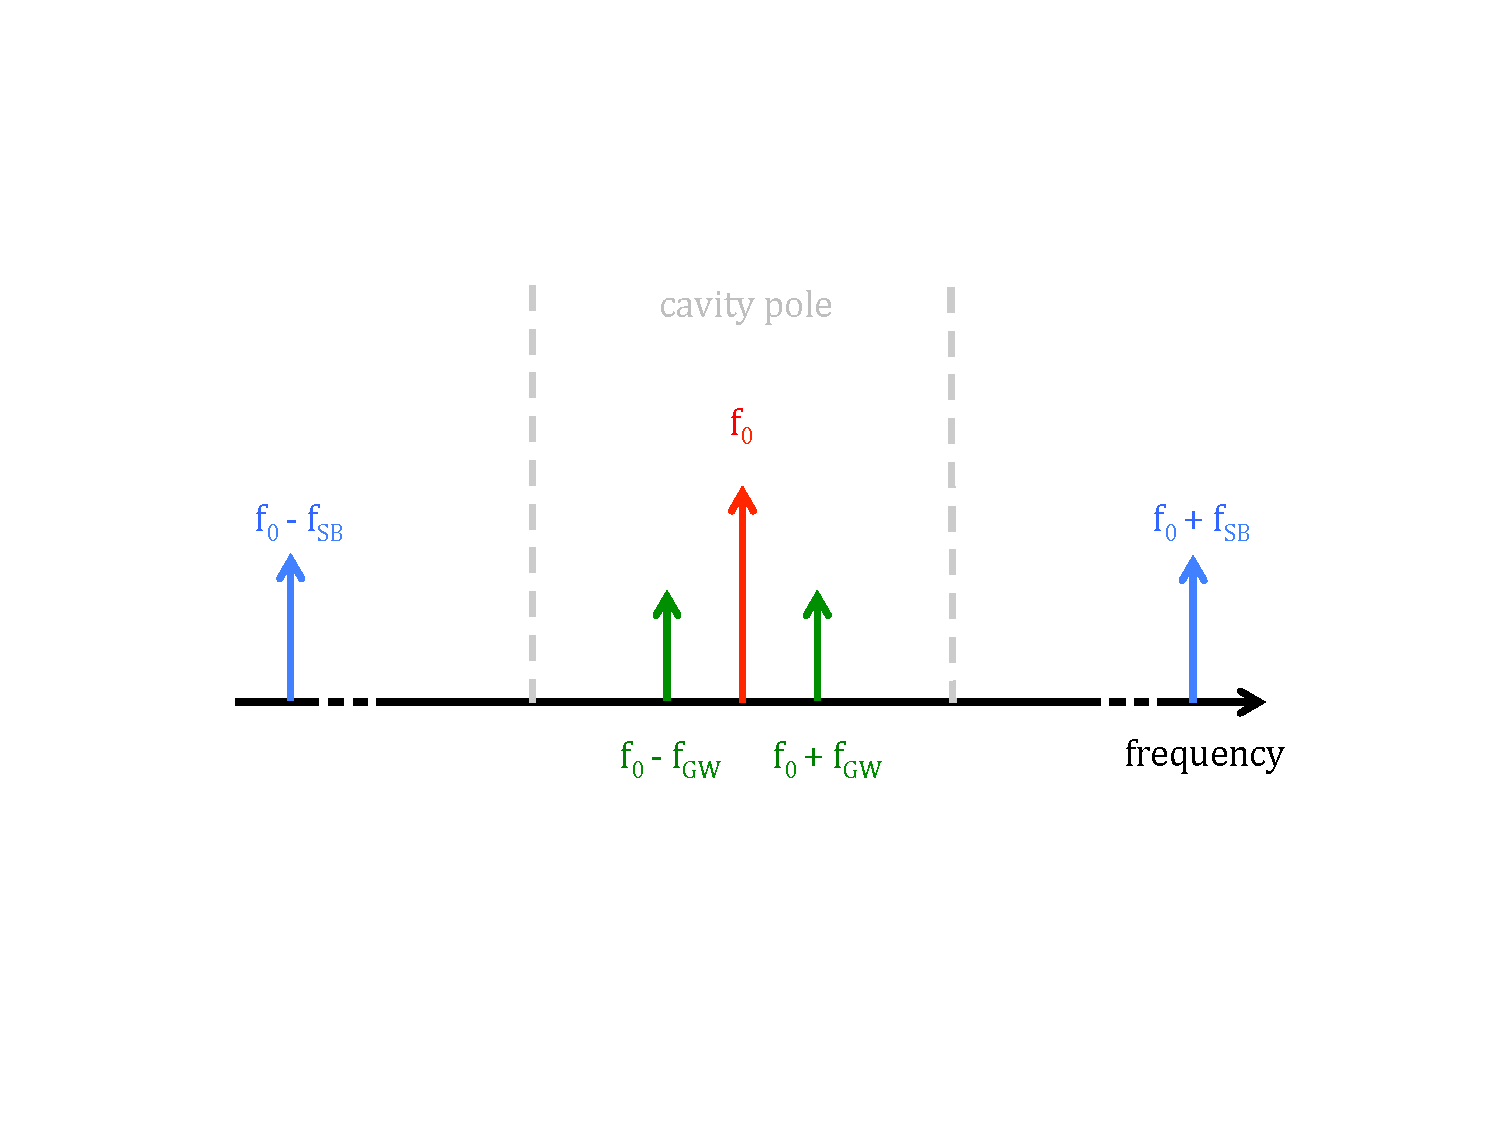
\includegraphics[width=\textwidth]{figures/introduction/omc-freq}
\caption[Sidebands and OMC cavity pole]{Frequency domain visualization of beam %
         at OMC. Grey dotted lines indicate the cavity pole. The gravitational %
         wave sidebands are within the cavity pole and are transmitted through %
         the OMC. The RF sidebands are in the MHz range and are rejected by the %
         OMC.}
\end{figure}\label{fig:omc-freq}

\section{Searching for Compact Binary Coalescences}

The PyCBC pipeline is designed to search for gravitational wave transients from compact binary
coalescences. It employs a matched-filter algorithm, which correlates
expected CBC
waveforms with detector data and assigns a ranking statistic, signal-to-noise ratio (SNR),
to every event that it finds. These events are referred to as triggers. In this algorithm,
the background noise power spectral density (PSD) is estimated by averaging individual
PSD measurements made over a 2048 second stride.

To perform this search, the matched-filter algorithm needs to know what to search for.
Before the search is run, a collection of expected CBC waveforms is generated using
the formalism of general relativity. Each of the expected waveforms is called a template and
the full collection of waveforms is referred to as the template bank. This template bank
is constructed to span the astrophysical parameter space included in the search. 
Each waveform is defined by the mass and spin of each compact
object in the binary system. It is often convenient to combine the effects of each
object's spin into one parameter called effective spin, $S_{eff}$,
which is the
mass-weighted spin of the system. $S_{eff}$ is defined as
\begin{equation}
S_{eff} = \frac{\boldsymbol{\chi_{1}}m_{1} + \boldsymbol{\chi_{2}}m_{2}}{m_{1} + m_{2}}
\end{equation}
where $\boldsymbol{\chi_{i}}$ is the dimensionless spin parameter and $m_{i}$ is the
mass for each compact object in the binary system.

The search algorithm is run separately at each interferometer and a set of single interferometer
triggers is generated. These sets are compared to search for any triggers that occurred in
coincidence between the two interferometers as would be expected from gravitational wave
signal. Any triggers that are found in coincidence between the two interferometers and
are recovered with the same source parameters represent a potential gravitational wave signal
and are labeled a foreground event.

To generate the background, all coincident triggers are removed
from the set of triggers generated for each interferometer, effectively removing all
potential gravitational wave signals from the data set. The remaining triggers are then
a realization of the background noise in each interferometer. These two sets of triggers,
one from each interferometer, are then time shifted by a duration longer than the
light travel time between the interferometers.
Since gravitational waves travel at the speed of light, this time shift ensures that the
two sets of triggers are astrophysically uncorrelated and do not contain any gravitational
wave signals. The coincidence test is then performed again with the time shifted triggers.
Since the trigger sets have been time shifted, the resulting coincident triggers
represent an example set of coincident triggers that should be expected from background noise alone.
A full distribution of background triggers is generated by performing this timeslide
technique every 0.1 seconds and iterating over all available data.

The statistical significance of any candidate gravitational wave is
evaluated by calculating the rate of background events from detector noise that are at least as
loud as the candidate event. This statistic is called the false alarm rate (FAR).
Any loud triggers that appear as the result of instrumental
transients will contribute to the tail of the background distribution and
the influence the measured false alarm rate.
The purpose of the data quality effort as a whole is thus two-fold: to ensure that the
search is using nominal, stationary
detector data in the background PSD estimation and to suppress the rate of loud events
that will pollute the search background.
There are two stages of
of data quality, gating and the $\chi^{2}$ signal consistency test, that are internal to the PyCBC search
pipeline.



\section{Detector Characterization}
